\chapter{Despacho económico a corto plazo.}
	\section{Despacho económico diario de generación. Mercado diario.}
		\textbf{Objetivo:} repartir la demanda total del sistema $P_D\,[MW]$ entre los generadores disponibles, de forma que el coste total de generación, en $\euro/MWh/\text{día}$, sea el mínimo posible, con las mínimas pérdidas en la red y menores emisiones de $CO_{2,eq}$.
		
		
		El \textbf{coste total de generación} es variable en cada hora, debido a que las centrales que intervienen tienen eficiencias y costes muy distintos.
		
		
		La resolución del despacho económico (D.E.) considera una serie de \textbf{restricciones técnicas} que limitan el uso de las centrales.
		
		
		Es necesario considerar la opción de \textbf{acoplar o desacoplar los grupos de generación} según la variación de la demanda.
		
		
		\textbf{Programación Horaria de Grupos Térmicos:} problema de operar un sistema de energía eléctrica a coste mínimo, debido a que
		
		\begin{itemize}
			\item[-] los costes fijos de operación de una central térmica pueden ser comparativamente altos, luego no es viable operar a un nivel de producción bajo \textrightarrow Desacoplar centrales cuando hay baja demanda.
			\item[-] las energías renovables ofertan a coste 0.
			\item[-] las centrales nucleares ofertan a coste casi 0 (por considerarse no regulables).
		\end{itemize}
		
		
		\textbf{Coordinación hidráulica:} contribuye a la disminución de los costes de generación en horas punta.
	
		\subsection{Problema de optimización.}
			Sea un sistema eléctrico con $m$ generadores y $n$ nudos. La resolución de un \textbf{flujo de carga óptimo} (OPF, Optimal Power Flow) consiste en elegir las potencias $P_{G_i}$ de los $m$ generadores disponibles y los módulos de las tensiones $U_i$ en los $n$ nudos, de forma que se minimice el coste total de generación $C_T$:
			
			\[C_T = \sum_{i = 1}^m C_i\,\left[\dfrac{\euro}{h}\right] \Rightarrow 
			OPF = \min{ \left\{ \sum_{i = 1}^n C_{G_i} (P_{G_i}) \right\} } \]
			
			
			Son problemas de \textbf{optimización lineal}, \textbf{lineal entera mixta} o \textbf{no lineal} cuando se tienen en cuenta las pérdidas eléctricas, sujetos a restricciones. 
			
		\subsection{Restricciones en la optimización.}
			Las potencias generadas por cada grupo deben estar comprendidas entre un \textbf{límite mínimo}, dado por la \textbf{turbina}, y un \textbf{máximo}, dado por el \textbf{generador}.
			
			
			El flujo de potencia activa y reactiva en cada línea no puede superar un valor máximo por motivos de la capacidad de la línea.
			
			
			La tensión y frecuencia en los nudos del sistema no debe quedar fuera de los límites impuestos por la calidad de suministro (en redes de transporte de 220-400 kV).
			
			\begin{figure}
					\begin{minipage}{0.5\textwidth}
					\begin{table}[H]
						\centering
						\begin{tabular}{cc}
							\textbf{Rango de} & \textbf{Periodo de tiempo}\\
							\textbf{tensión} & \textbf{de funcionamiento}\\
							\hline
							$0.85-0.9\,p.u.$ & 60 minutos\\
							$0.9-1.0875\,p.u.$ & Ilimitado\\
							$1.0875-1.1\,p.u.$ & 60 minutos
						\end{tabular}
						%\caption{Tiempos máximos de caídas de tensión en redes de transporte.}
						\label{tab:tiemposCdt}
					\end{table}
				\end{minipage}
				\begin{minipage}{0.5\textwidth}
					\begin{table}[H]
						\centering
						\begin{tabular}{cc}
							\textbf{Rango de} & \textbf{Periodo de tiempo}\\
							\textbf{frecuencias} & \textbf{de funcionamiento}\\
							\hline
							$47.5-48.5\,Hz$ & 30 minutos\\
							$48.5-49.0\,Hz$ & Ilimitado\\
							$49.0-51.0\,Hz$ & Ilimitado\\
							$51.0-51.5\,Hz$ & 30 minutos
						\end{tabular}
						%\caption{Tiempos máximos de caídas de tensión en redes de transporte.}
						\label{tab:tiemposfrecuencias}
					\end{table}	
				\end{minipage}	
			\end{figure}	
			
	\section{Unidades térmicas generadoras. Curva de consumo.}
			Una central térmica generadora queda descrita por:
			\begin{itemize}
				\item Cantidad de calor de entrada requerido: $H_{G_i}\,\left[\dfrac{MJ}{h}\right]$.
				\item Cantidad de energía eléctrica entregada (trifásica): $P_{G_i}\,[MW]$.
			\end{itemize}
			
			\[H_{G_i} = \alpha_i + \beta_i \cdot P_{G_i} + \gamma_i \cdot P_{G_i}^2\,\left[\dfrac{MJ}{h}\right]\]
			
			\begin{itemize}
				\item $\alpha_i$ son los costes fijos $[\euro/h]$ de operación (salarios de los trabajadores) y consumo de combustible de autoconsumo cuando la producción es 0.
				\item $\beta_i$ y $\gamma_i$ son parámetros positivos que caracterizan la dependencia de la curva de costes o de consumo con su nivel de generación.
			\end{itemize}
			
			\begin{figure}[H]
				\begin{minipage}{0.4\textwidth}
					\begin{figure}[H]
						\centering
							\begin{circuitikz}[scale = 0.5]
								\tikzstyle{every node}=[font=\normalsize]
								\draw [->, >=Stealth] (3.5,10.25) -- (3.5,16)node[pos=1,right]{$H_{G_i}\,[MW/h]$};
								\draw [->, >=Stealth] (3.5,10.25) -- (9.5,10.25)node[pos=1,right]{$P_{G_i}\,[MW]$};
								\draw [ color={rgb,255:red,0; green,128; blue,255}, short] (3.5,11.25) .. controls (6.5,11.5) and (8,11.75) .. (9,15.25);
								\draw [dashed] (4.5,11.25) -- (4.5,10.25)node[pos=1,below]{$P_{G_i}^{min}$};
								\draw [dashed] (8.5,13.75) -- (8.5,10.25)node[pos=1,below]{$P_{G_i}^{max}$};
							\end{circuitikz}
						
						\label{fig:my_label}
					\end{figure}
				\end{minipage}
				\begin{minipage}{0.6\textwidth}
					Esta es la función que define la \textbf{curva de consumo}, y expresa la cantidad de combustible consumido por hora en función de la producción eléctrica. Mide la eficiencia de la unidad de producción. Puede ser continua o a tramos.
					
					\vspace{0.25cm}
					Esta curva se obtiene de pruebas que se le realizan al grupo turbina-generador para varios niveles de salida: 100, 75, 50 y 25\%, por ejemplo.
				\end{minipage}
			\end{figure}
	
		\subsection{Característica de coste de las unidades térmicas generadoras.}
			Multiplicando la cantidad de calor $H_{G_i}$ por el coste de combustible se obtiene la función de coste total de cada unidad de producción $C_i(P_{G_i})$, en $\euro/h$ y en función de $P_{G_i}$.
			
			\begin{figure}[H]
				\begin{minipage}{0.4\textwidth}
					\begin{figure}[H]
						\centering
						\begin{circuitikz}[scale = 0.5]
							\tikzstyle{every node}=[font=\normalsize]
							\draw [->, >=Stealth] (3.5,10.25) -- (3.5,16)node[pos=1,right]{$C_i(P_{G_i})\,[\euro/h]$};
							\draw [->, >=Stealth] (3.5,10.25) -- (9.5,10.25)node[pos=1,right]{$P_{G_i}\,[MW]$};
							\draw [ color={rgb,255:red,0; green,128; blue,255}, short] (3.5,11.25) .. controls (6.5,11.5) and (8,11.75) .. (9,15.25);
							\draw [dashed] (4.5,11.25) -- (4.5,10.25)node[pos=1,below]{$P_{G_i}^{min}$};
							\draw [dashed] (8.5,13.75) -- (8.5,10.25)node[pos=1,below]{$P_{G_i}^{max}$};
						\end{circuitikz}
						
						\label{fig:my_label}
					\end{figure}
				\end{minipage}
				\begin{minipage}{0.6\textwidth}
					El coste total incluye un coste fijo (que no contiene coste de inversión), costes de operación fijos, consumos propios y costes variables de O\&M, combustible, emisiones de $CO_2$, etc. Los costes variables son dependientes de la potencia activa que entrega el generador. Las centrales hidráulicas tienen una curva similar en función del caudal turbinado.
					
					\vspace{0.25cm}
					Si la curva de consumo es una función cuadrática admite soluciones analíticas:
					\[C_i(P_{G_i}) = \alpha_i + \beta_i\cdot P_{G_i} + \gamma_i\cdot P_{G_i}^2\]
				\end{minipage}
			\end{figure}
			
		\subsection{Conversión de la curva de consumo específico a curva de costes.}
			$1\,th = 1.162\,kWh = 1000\,kcal$
			
			$1\,kWh = 0.86\,th$
			
			$1\,tep = 11.627\,MWh = 10^4\,th$
			
			$1\,kJ = 9.5\,th$
			
		\subsection*{Ejemplo.}
			Una central térmica de carbón, con un PCI de $6050\,th/t$ tiene un coste de $37.91\,\euro/t$. Obtener la curva de coste del generador.
			\[C_1\,\left[\dfrac{\euro}{h}\right] = \dfrac{H_1\,\left[\dfrac{th}{h}\right]}{6050\,\left[\dfrac{th}{t}\right]} \cdot 37.91\,\left[\dfrac{\euro}{t}\right] = 426.56 + 10.756\cdot P_{G_1} + 0.0031\cdot P_{G_1}^2\]
			
		\subsection{Restricciones técnicas de la curva de coste o consumo.}
			\begin{itemize}
				\item Límites operativos:
				\begin{itemize}
					\item Potencia mínima (por caldera y turbina).
					\item Potencia máxima (por generador síncrono).
				\end{itemize}
				
				\item Tiempo mínimo de operación.
				\item Tiempo mínimo de arranque.
				\item Tiempo de respuesta entre intervalos horarios: Rampa de subida y bajada [MW/h].
				\item Coste de arranque.
				\item Coste de parada.
				\item Penalizaciones por emisiones de $CO_2$.
			\end{itemize}
			
		\subsection{Consumo específico o \textit{Heat Rate} (H.R.).}
			Es la medida del rendimiento de una central termoeléctrica. Se define por el cociente entre la energía térmica aportada en forma de combustible y la energía generada en bornes del generador.
			
			\[HR = \dfrac{H_{G_i}}{P_{G_i}} = \dfrac{\alpha_i}{P_{G_i}} + \beta_i + \gamma_i\cdot P_{G_i}\]
			
			La máxima eficiencia de la unidad se obtiene en el mínimo de la función HR, que se da para valores próximos a la potencia máxima del generador.
			
			\begin{figure}[H]
				\begin{minipage}{0.35\textwidth}
					\begin{figure}[H]
						\centering
						\begin{circuitikz}[scale = 0.65]
							\tikzstyle{every node}=[font=\normalsize]
							\draw [->, >=Stealth] (3.5,10.25) -- (3.5,16)node[pos=1,right]{$H\!R\,\left[\dfrac{MJ}{MWh}\right]$};
							\draw [->, >=Stealth] (3.5,10.25) -- (9.5,10.25)node[pos=1.1,above]{$P_{G_i}\,[MW]$};
							\draw [ color={rgb,255:red,0; green,128; blue,255}, short] (4.5,15.25) .. controls (6,11.5) and (8,11.85) .. (8.5,13.25);
							\draw [dashed] (4.5,15.25) -- (4.5,10.25)node[pos=1,below]{$P_{G_i}^{min}$};
							\draw [dashed] (8.5,13.25) -- (8.5,10.25)node[pos=1,below]{$P_{G_i}^{max}$};
							\draw [dashed] (7.25,12.25) -- (7.25,10.25)node[pos=1,below]{$P_{ef}$};
							\draw [dashed] (7.25,12.25) -- (3.5,12.25);
							\draw (7.25,12.25) to[short, -*] (7.25,12.25);
						\end{circuitikz}
						
						\label{fig:my_label}
					\end{figure}
				\end{minipage}
				\begin{minipage}{0.65\textwidth}
					\begin{figure}[H]
						\centering
						\begin{circuitikz}[scale = 0.5]
							\tikzstyle{every node}=[font=\normalsize]
							\draw [->, >=Stealth] (3.5,10.25) -- (3.5,16)node[pos=1,right]{$\eta\,[\%]$};
							\draw [->, >=Stealth] (3.5,10.25) -- (9.5,10.25)node[pos=1.1,above]{$P_{G_i}\,[MW]$};
							\draw [ color={rgb,255:red,0; green,128; blue,255}, short] (4.25,11.25) .. controls (4.75,13.75) and (6.5,15) .. (8.75,15);
							\draw [->, >=Stealth] (12.5,10.25) -- (12.5,16.25)node[pos=1,right]{$H\!R\,\left[\dfrac{MJ}{MWh}\right]$};
							\draw [->, >=Stealth] (12.5,10.25) -- (18.25,10.25)node[pos=1.1,above]{$P_{G_i}\,[MW]$};
							\draw [ color={rgb,255:red,0; green,128; blue,255}, short] (13.5,15) .. controls (14,12.5) and (15.25,11.5) .. (17.5,11.25);
						\end{circuitikz}
						
						\label{fig:my_label}
					\end{figure}
				\end{minipage}
			\end{figure}
			
			\[\eta = \dfrac{3600}{H\!R}\,\left[\dfrac{MWh_e}{MWh_t}\right] \qquad 
			H\!R = \dfrac{3600}{\eta}\,\left[\dfrac{MJ}{MWh}\right]\]
			
		\newpage
		\subsection*{Ejemplo. Cálculo del HR para una turbina de gas.}
			\textbf{Ojo:} el HR de la turbina determinado mediante pruebas es distinto del $H\!R_{ISO}$ que proporciona el fabricante.
			
			\begin{figure}[H]
				\centering
				\includegraphics[width=0.7\linewidth]{res/tema5/turbinaGas}
				\label{fig:turbinagas}
			\end{figure}
			\vspace{-1cm}
			\begin{figure}[H]
				\begin{minipage}{0.325\textwidth}
					\begin{table}[H]
						\renewcommand{\arraystretch}{1.2}
						\centering
						\begin{tabular}{lcc}
							\multicolumn{3}{c}{\textbf{Datos}}\\
							\hline
							\textbf{Mag.} & \textbf{Uds.} & \textbf{Valor}\\
							\hline
							$T_{amb}$ & $^\circ C$ & 15\\
							\hline
							$P_{atm}$ & $mbar$ & 1013\\
							\hline
							\multirow{2}{*}{$H\!R_{ISO}$} & \multirow{2}{*}{$\dfrac{kJ}{kWh}$} & \multirow{2}{*}{9526}\\
							&&\\
							\hline
							\multirow{2}{*}{PCI} & \multirow{2}{*}{$\dfrac{MJ}{Nm^3}$} & \multirow{2}{*}{35.5}\\
							&&\\
							\hline
							$P_{e,\,neta}$ & \multirow{2}{*}{$MW$} & \multirow{2}{*}{240}\\
							(ISO)&&
						\end{tabular}
					\end{table}
				\end{minipage}
				\begin{minipage}{0.675\textwidth}
					$\eta_{ISO} = \dfrac{3600\,\dfrac{kJ}{kWh}}{H\!R_{ISO}} = \dfrac{3600\,\dfrac{kJ}{kWh}}{9526\,\dfrac{kJ}{kWh}}\cdot 100 = 37.7\%$
				
					$\eta_{ISO} = \dfrac{P_{neta,\,ISO}}{P_{GN}}$
					
					$P_{GN} = \dfrac{240}{0.377} = 636.60\,MW = \text{Vol}_{GN}\,\left[\dfrac{Nm^3}{h}\right] \cdot PCI_{GN}\,\left[\dfrac{MJ}{Nm^3}\right]$
					
					$\text{Vol}_{GN} = \dfrac{636.60}{35.5}\cdot 3600\,\dfrac{s}{h} = 64557.1\,\dfrac{Nm^3}{h}$
				\end{minipage}
			\end{figure}
			
			Energía aportada por el GN: 
			
			$\qquad E = \text{Vol}_{GN} \cdot PCI_{GN} = 64557.1 \cdot 35.5 = 2.292\,\dfrac{GJ}{h}$
			
			\vspace{0.2cm}
			Factores de corrección en la potencia por variación de temperatura y presión atmosférica:
			
			
			Condiciones de funcionamiento de la turbina de gas en la central: $T=16^\circ C$ y $P=900\,mbar$
			
			$\qquad P_{neta,\,ISO} = \dfrac{P_{neta,\,sitio}}{f_T \cdot f_P}$
			
			$\qquad f_P = \dfrac{900}{1013} = 0.888;\quad\quad f_T = \dfrac{15}{16} = 0.9375$
			
			$\qquad P_{sitio} = \dfrac{240\,MW}{0.9375 \cdot 0.888} = 199.8\,MW$
			
			\vspace{0.25cm}
			Heat Rate en el sitio de la instalación:
			
			\vspace{0.2cm}
			$\qquad H\!R_{ISO} = \dfrac{H\!R_{sitio}}{F_{TH}\,(\text{dato})}$
			
			$\qquad H\!R_{sitio} = 9.526 \dfrac{kJ}{kWh}\cdot 1.01 = 9.621.26 \dfrac{kJ}{kWh}$
			
			\vspace{0.25cm}
			Rendimiento:
			
			\vspace{0.2cm}
			$\qquad \eta_{sitio} = \dfrac{3600 \dfrac{kJ}{kWh}}{H\!R_{sitio}} =
				\dfrac{3600 \dfrac{kJ}{kWh}}{9621.26 \dfrac{kJ}{kWh}} \cdot 100 = 37.4\%$
				
			$\qquad \eta_{sitio} = \dfrac{P_{neta,\,sitio}}{P_{GN}}$
			
			$\qquad P_{GN} = \dfrac{199.8}{0.374} = 534.22\,MW = \text{Vol}_{GN}\,\left[\dfrac{Nm^3}{h}\right] \cdot PCI_{GN}\,\left[\dfrac{MJ}{Nm^3}\right]$
			
			\vspace{0.25cm}
			Energía aportada por el GN:
			
			$\qquad E = \text{Vol}_{GN} \cdot PCI_{GN} = 54174.88 \cdot 35.5 = 1.923\,\dfrac{GJ}{h}$
	
			\newpage
			
		\subsection*{Ejemplo. Cálculo del HR de dos unidades térmicas de carbón.}
			Sean dos unidades térmicas que queman carbón con sus respectivas curvas de consumo
			específico y limites de funcionamiento:
			
			\begin{figure}[H]
				\begin{minipage}{0.6\textwidth}
					\begin{figure}[H]
						\centering
						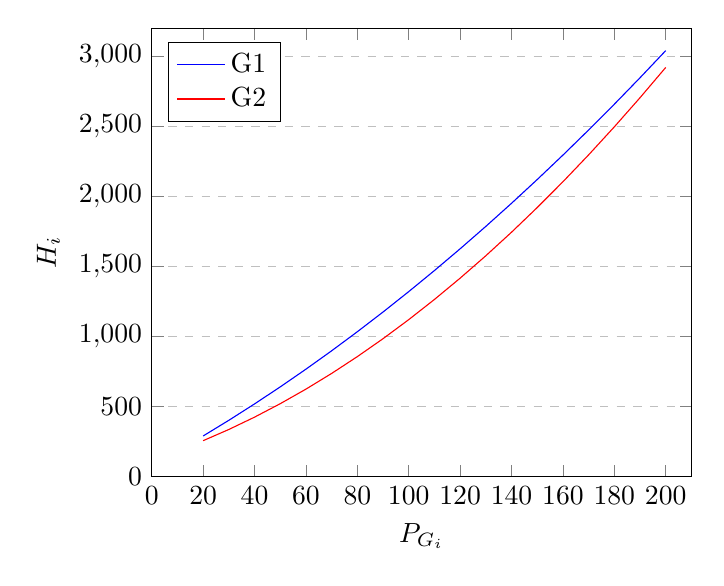
\begin{tikzpicture}
							\begin{axis}[
								xlabel={$P_{G_i}$},
								ylabel={$H_i$},
								xmin=0, xmax=210,
								ymin=0, ymax=3200,
								xtick={0,20,40,60,80,100,120,140,160,180,200,220},
								ytick={0,500,1000,1500,2000,2500,3000,3500},
								legend pos=north west,
								ymajorgrids=true,
								grid style=dashed,
								]
								
								\addplot[
								color=blue,
								]
								coordinates {
									(20,289.6)
									(30,401.6)
									(40,518.4)
									(50,640)
									(60,766.4)
									(70,897.6)
									(80,1033.6)
									(90,1174.4)
									(100,1320)
									(110,1470.4)
									(120,1625.6)
									(130,1785.6)
									(140,1950.4)
									(150,2120)
									(160,2294.4)
									(170,2473.6)
									(180,2657.6)
									(190,2846.4)
									(200,3040)
								};
								\addlegendentry{G1}
								
								\addplot[
								color=red,
								]
								coordinates {
									(20,256)
									(30,336)
									(40,424)
									(50,520)
									(60,624)
									(70,736)
									(80,856)
									(90,984)
									(100,1120)
									(110,1264)
									(120,1416)
									(130,1576)
									(140,1744)
									(150,1920)
									(160,2104)
									(170,2296)
									(180,2496)
									(190,2704)
									(200,2920)						
								};
								\addlegendentry{G2}
								
							\end{axis}
						\end{tikzpicture}
					\end{figure}
				\end{minipage}
				\begin{minipage}{0.4\textwidth}
					\begin{table}[H]
						\begin{tabular}{c}
							$H_1(P_{G_1}) = 80 + 10P_{G_1} + 0.024P_{G_1}^2\,\left[\dfrac{GJ}{h}\right]$\\ 
							$20\,MW \leq P_{G_1} \leq 100\,MW$\\
							\\
							\hline
							\\
							$H_2(P_{G_2}) = 120 + 6P_{G_2} + 0.04P_{G_2}^2\,\left[\dfrac{GJ}{h}\right]$\\
							$20\,MW \leq P_{G_2} \leq 100\,MW$
						\end{tabular}
					\end{table}
				\end{minipage}
			\end{figure}
			
			\begin{figure}[H]
				\begin{minipage}{0.6\textwidth}
					\begin{figure}[H]
						\centering
						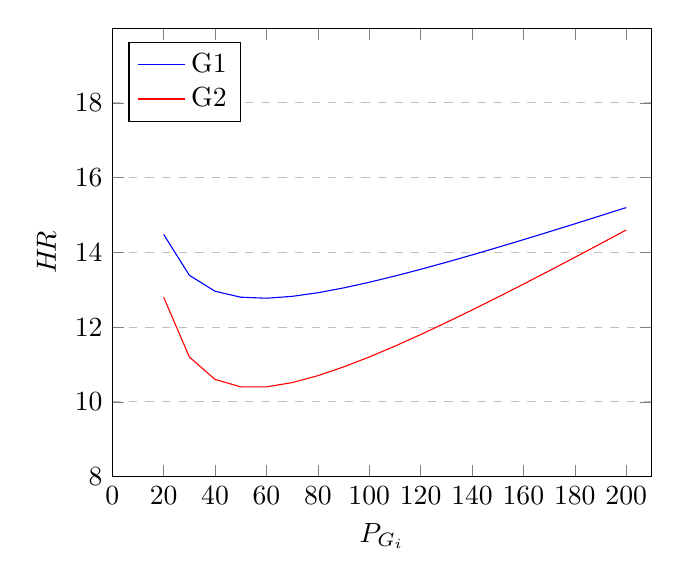
\begin{tikzpicture}
							\begin{axis}[
								xlabel={$P_{G_i}$},
								ylabel={$H\!R$},
								xmin=0, xmax=210,
								ymin=8, ymax=20,
								xtick={0,20,40,60,80,100,120,140,160,180,200,220},
								ytick={8,10,12,14,16,18},
								legend pos=north west,
								ymajorgrids=true,
								grid style=dashed,
								]
								
								\addplot[
								color=blue,
								]
								coordinates {
									(20	,14.48)
									(30	,13.38666667)
									(40	,12.96)
									(50	,12.8)
									(60	,12.77333333)
									(70	,12.82285714)
									(80	,12.92)
									(90	,13.04888889)
									(100,	13.2)
									(110,	13.36727273)
									(120,	13.54666667)
									(130,	13.73538462)
									(140,	13.93142857)
									(150,	14.13333333)
									(160,	14.34)
									(170,	14.55058824)
									(180,	14.76444444)
									(190,	14.98105263)
									(200,	15.2)
								};
								\addlegendentry{G1}
								
								\addplot[
								color=red,
								]
								coordinates {
									(20	,12.8)
									(30	,11.2)
									(40	,10.6)
									(50	,10.4)
									(60	,10.4)
									(70	,10.51428571)
									(80	,10.7)
									(90	,10.93333333)
									(100,	11.2)
									(110,	11.49090909)
									(120,	11.8)
									(130,	12.12307692)
									(140,	12.45714286)
									(150,	12.8)
									(160,	13.15)
									(170,	13.50588235)
									(180,	13.86666667)
									(190,	14.23157895)
									(200,	14.6)
									
								};
								\addlegendentry{G2}
								
							\end{axis}
						\end{tikzpicture}
					\end{figure}
				\end{minipage}
				\begin{minipage}{0.4\textwidth}
					El Heat Rate será la relación entre el consumo de energía (GJ) y la energía producida (MWh).
					
					\vspace{0.25cm}
					Se observa que en $P_G \approx 50\,MW$ se alcanzan los puntos de HR mínimo.
				\end{minipage}
			\end{figure}		
		
		\begin{figure}[H]
			\begin{minipage}{0.6\textwidth}
				\begin{figure}[H]
					\centering
					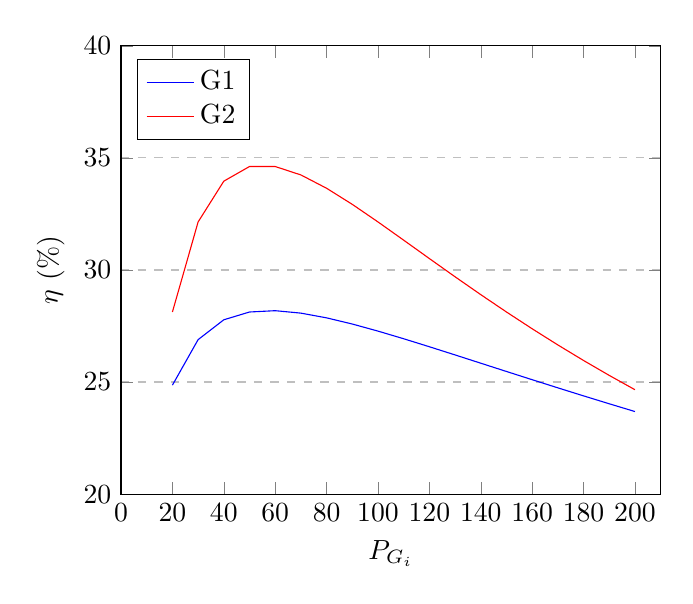
\begin{tikzpicture}
						\begin{axis}[
							xlabel={$P_{G_i}$},
							ylabel={$\eta$ (\%)},
							xmin=0, xmax=210,
							ymin=20, ymax=40,
							xtick={0,20,40,60,80,100,120,140,160,180,200,220},
							ytick={20,25,30,35,40},
							legend pos=north west,
							ymajorgrids=true,
							grid style=dashed,
							]
							
							\addplot[
							color=blue,
							]
							coordinates {
								(20	,24.86187845)
								(30	,26.89243028)
								(40	,27.77777778)
								(50	,28.125)
								(60	,28.18371608)
								(70	,28.07486631)
								(80	,27.86377709)
								(90	,27.58855586)
								(100,	27.27272727)
								(110,	26.93144723)
								(120,	26.57480315)
								(130,	26.20967742)
								(140,	25.84085316)
								(150,	25.47169811)
								(160,	25.10460251)
								(170,	24.74126779)
								(180,	24.38290187)
								(190,	24.03035413)
								(200,	23.68421053)
								
							};
							\addlegendentry{G1}
							
							\addplot[
							color=red,
							]
							coordinates {
								(20	,28.125      )
								(30	,32.14285714 )
								(40	,33.96226415 )
								(50	,34.61538462 )
								(60	,34.61538462 )
								(70	,34.23913043 )
								(80	,33.64485981 )
								(90	,32.92682927 )
								(100,	32.14285714)
								(110,	31.32911392)
								(120,	30.50847458)
								(130,	29.69543147)
								(140,	28.89908257)
								(150,	28.125     )
								(160,	27.37642586)
								(170,	26.65505226)
								(180,	25.96153846)
								(190,	25.29585799)
								(200,	24.65753425)
								
								
							};
							\addlegendentry{G2}
							
						\end{axis}
					\end{tikzpicture}
				\end{figure}
			\end{minipage}
			\begin{minipage}{0.4\textwidth}
				Como un $1\,MWh$ equivale a $3.6\,GJ$ se pueden calcular las eficiencias de cada unidad, dividiendo la
				equivalencia entre el valor del HR:
				
				\[\eta\,(\%) = \dfrac{3.6\,\left[\dfrac{GJ}{MWh}\right]\cdot P_{G_i}\,[MW]}{H_i\,\left[\dfrac{GJ}{h}\right]}\]
			\end{minipage}
		\end{figure}
		
	\newpage
		
	\section{Centrales hidráulicas. Curvas de coste y consumo.}
		\subsection{Curva de consumo específico de una central hidráulica de embalse.}
			\begin{figure}[H]
				\begin{minipage}{0.5\textwidth}
					Volumen de agua a desembalsar en un periodo considerado:
					\[P_h = P_h(Q,\,H)\,[MW]\]
					
					$Q \, \left[\dfrac{m^3}{s}\right]$ se puede mantener constante durante un periodo de tiempo.
					
					$H \, \left[m\right]$: salto. Variable a medida que se vacía el embalse.
					
					\vspace{0.5cm}
					Consumo de caudal en función del la potencia:
					\[Q(P_h) = \gamma_h P_h^2 + \beta_h P_h + \alpha_h\,\left[\dfrac{m^3}{h}\right]\]
					
					Restricciones:
					\begin{itemize}
						\item Régimen de lluvias.
						\item Potencia mínima técnica y potencia máxima: $P_{min} \leq P_h \leq P_{max}\,[MW]$
						\item Restricciones en el uso de los embalses.
						\item Tamaño de los embalses y acoplamiento entre ellos.
						\item Volumen de agua almacenado.
					\end{itemize}
				\end{minipage}
				\begin{minipage}{0.5\textwidth}
					\begin{figure}[H]
						\centering
						\begin{circuitikz}[scale = 0.95]
							\tikzstyle{every node}=[font=\normalsize]
							\draw [->, >=Stealth] (6.75,13.25) -- (6.75,17)node[pos=1,right]{$Q\,\left[\dfrac{m^3}{h}\right]$};
							\draw [->, >=Stealth] (6.75,13.25) -- (11.25,13.25)node[pos=1,above]{$P\,[MW]$};
							\draw [ color={rgb,255:red,0; green,128; blue,255}, short] (7.25,14.5) .. controls (10,15.25) and (9.75,15.5) .. (10.25,16.25);
							\draw [ color={rgb,255:red,0; green,128; blue,255}, dashed] (7.25,14.25) .. controls (10,15) and (9.75,15.5) .. (10.25,16);
							\draw [ color={rgb,255:red,0; green,128; blue,255}, dashed] (7.25,14) .. controls (10.5,15.25) and (9.75,15.25) .. (10.25,15.75);
							\draw [dashed] (10.25,16.25) -- (10.25,13.25)node[pos=1,below]{$P_{max}$};
							\draw [dashed] (7.25,14.5) -- (7.25,13.25)node[pos=1,below]{$P_{min}$};
							\node [font=\normalsize, rotate around={-360:(0,0)}] at (8.75,12.5) {Curva de entrada/salida};
							\draw [ color={rgb,255:red,0; green,128; blue,255}, ->, >=Stealth] (9.9,16.5) -- (9.75,15.5)node[pos=0,above]{Altura de salto fija};
							\draw [ color={rgb,255:red,0; green,128; blue,255}, ->, >=Stealth] (8.2,15.5) -- (7.75,14.2)node[pos=0,above]{Altura variable};
							\draw [ color={rgb,255:red,0; green,128; blue,255}, ->, >=Stealth] (8.2,15.5) -- (8,14.5);
							\draw [ color={rgb,255:red,0; green,128; blue,255}, ->, >=Stealth] (8.2,15.5) -- (8.25,14.8);
						\end{circuitikz}
						
						\label{fig:my_label}
					\end{figure}
					\begin{figure}[H]
						\centering
						\begin{circuitikz}[scale = 0.95]
							\tikzstyle{every node}=[font=\normalsize]
							\draw [->, >=Stealth] (6.75,13.25) -- (6.75,17)node[pos=1,right]{$C_{incr}\,\left[\dfrac{m^3}{MWh}\right]$};
							\draw [->, >=Stealth] (6.75,13.25) -- (11.25,13.25)node[pos=1,above]{$P\,[MW]$};
							\draw [ color={rgb,255:red,0; green,128; blue,255}, short] (7.25,14.5) .. controls (9.5,14.75) and (9.75,15) .. (10.25,15.25);
							\draw [dashed] (10.25,15.25) -- (10.25,13.25)node[pos=1,below]{$P_{max}$};
							\draw [dashed] (7.25,14.5) -- (7.25,13.25)node[pos=1,below]{$P_{min}$};
							\node [font=\normalsize, rotate around={-360:(0,0)}] at (8.75,12.5) {Consumos marginales};
						\end{circuitikz}
						
						\label{fig:my_label}
					\end{figure}
				\end{minipage}
			\end{figure}
			
		\subsection{Curva de coste de una central hidráulica de embalse.}
			El volumen de agua embalsada corresponde al \textbf{coste de oportunidad} del sistema. Reservan el agua para turbinarla
			en horas punta, y la central cobra según el precio fijado en esa hora.
			
			
			Para un periodo de operación de una hora, el coste asociado al volumen de agua turbinado queda
			expresado por una ecuación cuadrática:
			\[C(V) = \gamma_h V^2 + \beta_h V + \alpha_h\,\left[\dfrac{\euro}{h}\right]\]
			
			Dado que la central hidráulica genera por hora $G \, \left[\dfrac{MW}{m^3/s}\right]$, es posible convertir el costo de operación en
			función de la potencia generada:
			
			\[Q\,\left[\dfrac{m^3}{h}\right] = \dfrac{V\,[m^3]}{3600\,\left[\dfrac{s}{h}\right]}\]
			
			
			Que generará una potencia:
			
			\[P_h\,[MW] = G\,\left[\dfrac{MW}{m^3/s}\right]\cdot \dfrac{V}{3600} \left[\dfrac{m^3}{s}\right]\]
			
			Y despejando y sustituyendo queda:
			
			\[C_h(V) = \gamma_h \cdot \Biggl(\dfrac{3600\cdot P_h\,[MW]}{G\,\left[\dfrac{MW}{m^3/s}\right]}\Biggl)^2 + \beta_h \cdot 
			\dfrac{3600\cdot P_h\,[MW]}{G\,\left[\dfrac{MW}{m^3/s}\right]} + \alpha_h\]
			
			Las centrales hidráulicas tienen unos costes fijos de operación $\alpha_h$ muy bajos $\left(\sim3\,\dfrac{\euro}{MWh}\right)$
			
		\subsection*{Ejemplo. Expresión de coste en función de la potencia.}
			Se conoce la curva de costes de una central hidráulica, donde se desprecia $\alpha_h$ y se generan $0.9\,\dfrac{MW}{m^3/s}$
			
			\[C_h(V) = 3.125\cdot 10^{-9}\,V^2 + 0.001625\,V\,\left[\dfrac{\euro}{h}\right]\]
			
			La expresión de coste en función de la potencia queda:
			\[V = \dfrac{3600\cdot P_h}{G} = 4000\cdot P_h\]
			\[C_h(P_h) = 0.05\,P_h^2 + 6.5\,P_h\,\dfrac{\euro}{h}\]
			
		\subsection{Central hidráulica reversible. Curva de consumo específico.}
			Consiste en turbinar en periodos de alto coste y bombear en bajo coste. Emplean turbinas reversibles y pueden funcionar con ciclo diario o semanal. Disponen de un salto constante y tienen un rendimiento constante:
			
			\[\eta = \dfrac{E_T}{E_B}\cdot 100 \approx 67\%\]
			
			\begin{figure}[H]
				\begin{minipage}{0.6\textwidth}
					\begin{figure}[H]
						\centering
						\begin{circuitikz}[scale = 0.9]
							\tikzstyle{every node}=[font=\normalsize]
							\draw [->, >=Stealth] (6.75,13.25) -- (6.75,17)node[pos=1,right]{$Q\,\left[\dfrac{m^3}{h}\right]$};
							\draw [->, >=Stealth] (2.25,13.25) -- (11.25,13.25)node[pos=1,above]{$P\,[MW]$};
							\draw [ color={rgb,255:red,0; green,128; blue,255}, short] (7.25,14.5) .. controls (10,15.5) and (9.75,15.5) .. (10.25,16.25);
							\draw [dashed] (10.25,16.25) -- (10.25,13.25)node[pos=1,below]{$P_{max}$};
							\draw [dashed] (7.25,14.5) -- (7.25,13.25)node[pos=1,below]{$P_{min}$};
							\node [font=\normalsize, rotate around={-360:(0,0)}] at (6.75,12.5) {Curva de entrada/salida};
							\draw [ color={rgb,255:red,0; green,128; blue,255}, short] (2.75,15.75) -- (3.25,15.5);
							\draw [dashed] (3,15.5) -- (3,13.25)node[pos=1,below]{$P_b$};
						\end{circuitikz}
						
						\label{fig:my_label}
					\end{figure}
				\end{minipage}
				\begin{minipage}{0.4\textwidth}
					Generación (potencia variable): 
					
					\[Q(P_h) = \gamma_h P_h^2 + \beta_h P_h + \alpha_h\,\left[\dfrac{m^3}{h}\right]\]
					
					Bombeo (potencia constante): 
					
					\[Q(P_b)\,\left[\dfrac{m^3}{h}\right]\]
				\end{minipage}
			\end{figure}
			
	
	\section{Coste total de producción del sistema eléctrico.}
		El coste total de producción de un sistema con $n$ generadores es la suma de los costes individuales:
		\[C(P_G) = \sum_{i=1}^{n} C_i(P_{G_i})\]
		
		Si la demanda total es $P_D^{\text{total}}$ y todos los generadores participan en el despacho económico,
		\[\sum_{i=1}^{n} P_{G_i} = P_D^{\text{total}} + P_{\text{pérdidas}}\]
		
		El despacho básico consiste en minimizar el coste de producción con respecto a las generaciones.
		\[\text{Objetivo: } \min{\left\{C_t = \sum_{i=1}^N C_i\right\}}\]
		
		\newpage
		\subsection{Restricciones en la producción de energía eléctrica.}
			\begin{itemize}
				\item Balance nodal: flujo de potencia, estabilidad y mantenimiento de las tensiones en los nudos.
				\item Restricciones de desigualdad en los generadores: $P_{G_i}^{\text{min}} \leq P_{G_i} \leq P_{G_i}^{\text{max}}$
				\item Límites operativos: capacidad de las líneas de transmisión.
				\item Restricciones de los sistemas hidráulicos: volumen de agua embalsada.
				\item Reserva rodante disponible.
				\item Mínimas pérdidas de energía activa en la red: $RI^2$ y $XI^2$.
				\item Límites de emisiones contaminantes.
				\item Consumo de una cuota mínima contratada de combustible (centrales de gas natural y carbón).
				\item Tiempos de respuesta ante una subida o bajada de cada generador.
				\item Costes de arranque y parada.
			\end{itemize}
			
		\subsection{Relajación Lagrangiana: optimización de funciónes sujetas a restricciones.}
			Sirve para encontrar los máximos y mínimos de funciones de
			varias variables sujetas a restricciones. Permite resolver el problema de coordinación hidrotérmica a
			corto plazo. Reduce el problema restringido con $n$ variables a uno sin restricciones de $n + k$ variables,
			donde $k$ es el número de restricciones.
			
			
			El objetivo es minimizar la función de coste $f(x_1, x_2,\dots x_n)$ sujeta a condiciones de igualdad $g_i(x_1,x_2,\dots x_n) = 0$ y desigualdad $g_i(x_1,x_2,\dots x_n) \leq 0$.
			
			
			Se crea una función disminuida introduciendo un vector de $k$ elementos $\lambda$:
			\[L = f - \sum_{i=1}^{k} \lambda_i g_i\]
			
			Los valores de $x_1,x_2,\dots x_n$ que minimizan $f$ sujeto a funciones $g$ son los que resuelven las ecuaciones
			\[\dfrac{\partial L}{\partial x_i} = \dfrac{\partial f}{\partial x_i} - \sum_{i=1}^{k} \lambda_i \dfrac{\partial g_i}{\partial x_i} = 0\]
			\[\dfrac{\partial L}{\partial \lambda_i} = g_i = 0\]
			
			\subsubsection{Propiedad del vector gradiente.}
				El vector gradiente en un punto es un vector perpendicular a la curva de nivel.
				Cuando las curvas de nivel de las funciones $f$ (función de costes) y $g$ (función de restricciones) son
				tangentes se consigue el punto óptimo de mínimo coste, y sus vectores gradientes son paralelos
				(tienen la misma dirección).
				
				\begin{figure}[H]
					\begin{minipage}{0.5\textwidth}
						\begin{figure}[H]
							\centering
							\begin{circuitikz}
								\tikzstyle{every node}=[font=\normalsize]
								\draw [->, >=Stealth] (6.75,13.25) -- (6.75,17)node[pos=1,right]{y};
								\draw [->, >=Stealth] (6.75,13.25) -- (11.25,13.25)node[pos=1,above]{x};
								\draw [ color={rgb,255:red,0; green,128; blue,255} , rotate around={61:(9.25,15.5)}] (9.25,15.5) ellipse (1.5cm and 2cm);
								\draw [ color={rgb,255:red,0; green,128; blue,255} , rotate around={61:(9,15.75)}] (9,15.75) ellipse (1cm and 1.5cm);
								\draw [ color={rgb,255:red,0; green,128; blue,255} , rotate around={61:(8.5,16)}] (8.5,16) ellipse (0.5cm and 0.75cm);
								\draw [ color={rgb,255:red,255; green,0; blue,0}, short] (11.25,17) .. controls (8.25,16.25) and (9.5,14.25) .. (7.5,13.25);
								\draw [ color={rgb,255:red,0; green,128; blue,255}, ->, >=Stealth] (9.25,15.5) -- (8.5,16);
								\draw [ color={rgb,255:red,255; green,0; blue,0}, ->, >=Stealth] (9.25,15.5) -- (10,15);
								\draw [ color={rgb,255:red,0; green,128; blue,0} , rotate around={61:(9.25,15.5)}, dashed] (9.25,15.5) ellipse (0.5cm and 1cm);
								\draw [ color={rgb,255:red,0; green,128; blue,0}, dashed] (9.25,16) -- (9.75,17.5);
								\node [font=\normalsize, color={rgb,255:red,0; green,128; blue,0}, rotate around={-360:(0,0)}] at (9.75,18.3) {Los vectores gradientes en el};
								\node [font=\normalsize, color={rgb,255:red,0; green,128; blue,0}, rotate around={-360:(0,0)}] at (9.75,18) {punto de tangencia están orientados};
								\node [font=\normalsize, color={rgb,255:red,0; green,128; blue,0}, rotate around={-360:(0,0)}] at (9.75,17.7) {en la misma dirección};
								\draw [ color={rgb,255:red,0; green,128; blue,255}, ->, >=Stealth] (8,15.75) -- (8.25,16);
								\draw [ color={rgb,255:red,0; green,128; blue,255}, ->, >=Stealth] (9,16.25) -- (8.5,16.25);
								\draw [ color={rgb,255:red,0; green,128; blue,255}, ->, >=Stealth] (8,16.5) -- (8.25,16.25);
								\draw [ color={rgb,255:red,0; green,128; blue,255}, ->, >=Stealth] (10.25,15) -- (10,15.5);
								\draw [ color={rgb,255:red,0; green,128; blue,255}, ->, >=Stealth] (9.75,16.5) -- (9.5,16.25);
								\draw [ color={rgb,255:red,0; green,128; blue,255}, ->, >=Stealth] (8,16.75) -- (8.25,16.5);
								\draw [ color={rgb,255:red,0; green,128; blue,255}, ->, >=Stealth] (8,15.25) -- (8.25,15.5);
								\draw [ color={rgb,255:red,0; green,128; blue,255}, ->, >=Stealth] (7.5,15.25) -- (7.75,15.5);
								\draw [ color={rgb,255:red,0; green,128; blue,255}, ->, >=Stealth] (10.25,14) -- (10,14.4);
								\draw [ color={rgb,255:red,0; green,128; blue,255}, ->, >=Stealth] (11,15.75) -- (10.5,15.5);
								\draw [ color={rgb,255:red,255; green,0; blue,0}, ->, >=Stealth] (8.5,14.25) -- (9,14);
								\draw [ color={rgb,255:red,255; green,0; blue,0}, ->, >=Stealth] (10,16.5) -- (10.25,16);
								\node [font=\footnotesize, color={rgb,255:red,255; green,0; blue,0}, rotate around={-360:(0,0)}] at (11.5,16.75) {$g(x,y)=c$};
								\node [font=\footnotesize, color={rgb,255:red,0; green,128; blue,255}, rotate around={-360:(0,0)}] at (9.9,13.75) {$f(x,y)=d_1$};
								\node [font=\footnotesize, color={rgb,255:red,0; green,128; blue,255}, rotate around={-360:(0,0)}] at (9.5,14.5) {$f(x,y)=d_2$};
								\node [font=\footnotesize, color={rgb,255:red,0; green,128; blue,255}, rotate around={-360:(0,0)}] at (7.6,14) {$f(x,y)=d_3$};
								\draw [ color={rgb,255:red,0; green,128; blue,255}, ->, >=Stealth, dashed] (7.5,14.25) -- (8.5,15.5);
							\end{circuitikz}
							
							\label{fig:my_label}
						\end{figure}
					\end{minipage}
					\begin{minipage}{0.5\textwidth}
						Cuando dos vectores apuntan en la misma dirección pero con distinto sentido	podemos multiplicar cualquiera de los dos por una constante $\lambda_0$ para obtener el otro.
						
						
						Si el punto $(x_0,\,y_0)$ cumple la condición de tangencia, entonces
						\[\vec \nabla f(x_0,\,y_0) = \lambda_0 \vec \nabla g(x_0,\,y_0)\]
						\[\lambda_0 = \text{multiplicador de Lagrange}\]
					\end{minipage}
				\end{figure}
				
			\subsubsection{Función lagrangiana.}
				\[L(x,y,\lambda) = f(x,y) - \lambda(g(x,y)-c)\]
				
				Condiciones de mínimo necesarias: $\vec \nabla L = 0 \Rightarrow$ puntos críticos de $L$ (mínimos o máximos).
				
			\subsubsection{Coste incremental de la generación.}
				Derivando la expresión de la curva de coste con respecto a $P_{G_i}$:
				\[C_i(P_{G_i}) = \alpha_i + \beta_i P_{G_i} + \gamma_i P_{G_i}^2\,\left[\dfrac{\euro}{h}\right]\]
				
				Se obtiene el valor del coste incremental $\lambda$, que corresponde a la ecuación de una recta de pendiente $2\gamma_i$ y ordenada en el origen $\beta_i$.
				\[CI_i(P_{G_i}) = \dfrac{dC_i(P_{G_i})}{dP_{G_i}} = \beta_i + 2\gamma_i P_{G_i} = \lambda\,\left[\dfrac{\euro}{MWh}\right]\]
				
				
				\begin{figure}[H]
					\begin{minipage}{0.65\textwidth}
						El objetivo es conseguir el mismo coste incremental $\lambda$ para todos los generadores. No siempre se podrá cumplir, sobre todo si los generadores trabajan en su límite de funcionamiento y el sistema tiene pérdidas.
						
						\vspace{0.25cm}
						El valor común de $\lambda$ será el coste total o marginal óptimo para ese tramo horario:
						\[\lambda = \dfrac{dC(P_G)}{dP_D^{total}}\, \left[\dfrac{\euro}{MWh}\right]\]
					\end{minipage}
					\begin{minipage}{0.35\textwidth}
						\begin{figure}[H]
							\centering
							\begin{circuitikz}[scale = 0.7]
								\tikzstyle{every node}=[font=\normalsize]
								\draw [->, >=Stealth] (5,10.75) -- (5,14.75);
								\draw [->, >=Stealth] (5,10.75) -- (9.5,10.75)node[pos=1,above]{$P_{G_i}$};
								\draw [ color={rgb,255:red,255; green,0; blue,0}, dashed] (5,12.75) -- (9.5,12.75)node[pos=0,left]{$\lambda$};
								\draw [ color={rgb,255:red,0; green,128; blue,255}, short] (5.25,12) -- (7.25,13.5)node[pos=1,above]{$G_A$};
								\draw [ color={rgb,255:red,0; green,128; blue,255}, short] (6.5,11.25) -- (8.25,14.75)node[pos=1,above]{$G_B$};
								\draw [ color={rgb,255:red,0; green,128; blue,255}, short] (6.75,11.25) -- (10,14)node[pos=1,above]{$G_C$};
								\draw [dashed] (6.25,12.75) -- (6.25,10.75)node[pos=1,below]{$P_A$};
								\draw [dashed] (7.25,12.75) -- (7.25,10.75)node[pos=1,below]{$P_B$};
								\draw [dashed] (8.5,12.75) -- (8.5,10.75)node[pos=1,below]{$P_C$};
							\end{circuitikz}
							
							\label{fig:my_label}
						\end{figure}
					\end{minipage}
				\end{figure}
				
				El coste total de producción de un sistema se reduce al mínimo cuando todas las unidades generadoras se cargan de modo que sus costes marginales son los mismos: $\lambda_1 = \lambda_2 = \dots = \lambda_n = \lambda$
				
				
			\subsubsection{Despacho económico óptimo.}
				Si dos generadores térmicos trabajan con costes incrementales distintos $(\lambda_1 \neq \lambda_2)$, siempre es posible realizar la reasignación de las potencias de un generador a otro obteniendo una disminución del coste total de generación.
				
				
				Si, por ejemplo, $\lambda_1 < \lambda_2$, ante un incremento de potencia el generador 1 será más económico y por tanto su incremento de potencia será mayor.
				
				\begin{figure}[H]
					\begin{minipage}{0.5\textwidth}
						\begin{figure}[H]
							\centering
							\begin{circuitikz}[scale = 0.75]
								\tikzstyle{every node}=[font=\normalsize]
								\draw [->, >=Stealth] (5,10.75) -- (5,14.75)node[pos=1,above]{$C_1(P_1)$};
								\draw [->, >=Stealth] (5,10.75) -- (9.5,10.75)node[pos=1,above]{$P_{G_1}$};
								\draw [ color={rgb,255:red,0; green,128; blue,255}, short] (6,12) .. controls (7.25,12.25) and (8.25,13) .. (9,14);
								\draw [short] (6,12) -- (7,12)node[pos=0.5,below]{$\Delta$ $P_1$};
								\draw [short] (6,12) -- (7,12.25);
								\draw [short] (7,12.25) -- (7,12)node[pos=0.5,right]{$\Delta$ $C_1$};
								\node [font=\normalsize, color={rgb,255:red,0; green,128; blue,255}] at (7,13.75) {$\lambda_1 = \dfrac{\Delta C_1}{\Delta P_1}$};
							\end{circuitikz}
							
							\label{fig:my_label}
						\end{figure}
					\end{minipage}
					\begin{minipage}{0.5\textwidth}
						\begin{figure}[H]
							\centering
							\begin{circuitikz}[scale = 0.75]
								\tikzstyle{every node}=[font=\normalsize]
								\draw [->, >=Stealth] (5,10.75) -- (5,14.75)node[pos=1,above]{$C_2(P_2)$};
								\draw [->, >=Stealth] (5,10.75) -- (9.5,10.75)node[pos=1,above]{$P_{G_2}$};
								\draw [ color={rgb,255:red,0; green,128; blue,255}, short] (6,12) .. controls (6.75,12.5) and (7.5,13) .. (7.75,14.5);
								\draw [short] (6,12) -- (7,12)node[pos=0.5,below]{$\Delta$ $P_2$};
								\draw [short] (6,12) -- (7,12.6);
								\draw [short] (7,12.6) -- (7,12)node[pos=0.5,right]{$\Delta$ $C_2$};
								\node [font=\normalsize, color={rgb,255:red,0; green,128; blue,255}] at (9,13.75) {$\lambda_2 = \dfrac{\Delta C_2}{\Delta P_2}$};
							\end{circuitikz}
							
							\label{fig:my_label}
						\end{figure}
					\end{minipage}
				\end{figure}
				
				Si existe una solución óptima, si la demanda varía una cantidad diferencial $dP_D^{total}$ los niveles de generación también varían de forma que exista un equilibrio:
				\[\sum_{i=1}^n P_{G_i} = P_D^{total}\]
				\[dC(P_G) = \sum_{i=1}^n dC_i(P_{G_i}) = \sum_{i=1}^n CI_i(P_{G_i})\,dP_{G_i} = \sum_{i=1}^n \lambda\, dP_{G_i} = \lambda \sum_{i=1}^n dP_{G_i} = \lambda dP_D^{total}\]
				
				
				Luego de las expresiones anteriores se deduce que $\uparrow P_G \Rightarrow \uparrow \lambda$ de forma lineal con la demanda, que se reparte de forma distinta entre todos los generadores.
				
		\subsection{Formulación general del problema de optimización.}
			\[C(P_G) = \sum_{i=1}^n C_i(P_{G_i})\]
			\[F.O. = \min{\left\{\sum_{i=1}^n C_{G_i}(P_{G_i})\right\}}\]
				
			Restricciones de igualdad y desigualdad:
			\[\sum_{i=1}^n P_{G_i} = P_D^{total} + P_{perd}\]
			\[P_{G_i}^{min} \leq P_{G_i} \leq P_{G_i}^{max}\]
			
			Función lagrangiana:
			\[L = \sum_{i=1}^{n} C_i(P_{G_i}) - \lambda \left(\sum_{i=1}^{g} P_{G_i} P_D\right)\]

	\section{Modelos de estudio del despacho económico.}
		\subsection{Modelo simple. Despacho económico sin pérdidas en la red y sin límites en la generación.}
			La función lagrangiana es:
			\[L(P_G,\,\lambda) = \sum_{i=1}^{n} C_i(P_{G_i}) - \lambda \left(\sum_{i=1}^{g} P_{G_i} P_D\right)\]
		
			Las condiciones necesarias de primer orden apra la solución del óptimo son:
			\[\dfrac{\partial L(P_{G_i},\,\lambda)}{\partial P_{G_i}} = CI_i(P_{G_i}) - \lambda = 0 \qquad \because CI_i(P_{G_i}) = \lambda\]
			
			\[\dfrac{\partial L(P_{G_i},\,\lambda)}{\partial \lambda} = - \sum_{i=1}^{n} P_{G_i} + P_D^{total} = 0 \qquad\because P_D^{total} = \sum_{i=1}^{n} P_{G_i}\]
			
		\subsection*{Ejemplo. Modelo simple de despacho económico.}	
			Determinar la potencia que debe entregar cada generador, el coste incremental y el coste total.
			
			
			\underline{Datos:}
			\begin{itemize}
				\item Curvas de coste de funcionamiento:
				\[C_1(P_{G_1}) = 900 + 45\, P_{G_1} + 0.01\, P_{G_1}^2\,\dfrac{UM}{h}\]
				\[C_2(P_{G_2}) = 2500 + 43\, P_{G_2} + 0.003\, P_{G_2}^2\,\dfrac{UM}{h}\]
				
				\item Carga total a suministrar:
				\[P_D = 700\,MW\]
			\end{itemize}
			
			
			\underline{Solución:}
			
			
			Se debe cumplir que $\lambda = CI_1 = CI_2$ y que $P_{G_1} + P_{G_2} = P_D$:
			\[
			\left.
			\begin{matrix}
				\lambda = CI_1 = 45+0.02\,P_1\\
				\lambda = CI_2 = 43+0.006\,P_2\\
				P_1 + P_2 = 700
			\end{matrix}
			\right\}
			\begin{matrix}
				P_1 = 84.6\,MW\\
				P_2 = 615.4\,MW\\
				\lambda = 46.69\,\dfrac{UM}{MWh}
			\end{matrix}
			\]
			
			Coste total de operación mínimo:
			\[C_T = C_1 + C_2 = 900 + 45\,P_1 + 0.01\,P_1^2+2500+43\,P_2+0.003\,P_2^2 = 34876.92\,\dfrac{UM}{h}\]
		
		\subsection{Modelo sin pérdidas y con límites de generación.}
			El mínimo teórico de la turbina y la potencia máxima del generador aportan restricciones adicionales al problema de optimización, que en la práctica resulta en la no igualdad de costes incrementales cuando algún generador alcanza el límite. En consecuencia, para una demanda concreta podrán coexistir en despacho económico generadores trabajando a un coste incremental superior al del sistema (con potencia mínima), coste incremental inferior al del sistema (con potencia máxima) y coste incremental igual al del sistema.
			
			
			La función lagrangiana es:
			\[L(P_G,\lambda) = \sum_{i=1}^{n} C_i(P_{G_i}) - \lambda \left(\sum_{i=1}^{n} P_{G_i} - P_D^{total}\right) - \sum_{i=1}^{n} \mu_i^{max} (P_{G_i} - P_{G_i}^{max}) - \sum_{i=1}^{n} \mu_i^{min} (P_{G_i} - P_{G_i}^{min})\]
			
			Condiciones necesarias de primer orden para la solución óptima:
			\[\dfrac{\partial L(P_{G_i},\lambda)}{\partial P_{G_i}} = CI_i(P_{G_i})-\lambda - \mu_i^{max}-\mu_i^{min} = 0\]
				
			\[\dfrac{\partial L(P_{G_i},\lambda)}{\partial \lambda} = -\sum_{i=1}^{n} P_{G_i} + P_D^{total} = 0\]
			
			
			Restricciones de desigualdad:
			
			$\mu_i^{max} \leq 0$ si $P_{G_i} = P_{G_i}^{max}$
			
			$\mu_i^{max} =    0$ si $P_{G_i} < P_{G_i}^{max}$
			
			$\mu_i^{min} \geq 0$ si $P_{G_i} = P_{G_i}^{min}$
			
			$\mu_i^{min} =    0$ si $P_{G_i} > P_{G_i}^{min}$
			
			
			\vspace{0.25cm}
			En el óptimo:
			
			$CI_i(P_{G_i}) = \lambda + \mu_i^{min} \geq \lambda$ \quad si $P_{G_i} = P_{G_i}^{min}$
			
			$CI_i(P_{G_i}) = \lambda$ \qquad \qquad \qquad \, si $P_{G_i}^{min} < P_{G_i} < P_{G_i}^{max}$
			
			$CI_i(P_{G_i}) = \lambda + \mu_i^{max} \geq \lambda$ \quad si $P_{G_i} = P_{G_i}^{max}$
			
			
			\vspace{0.5cm}
			Los generadores que operan en su límite inferior tienen un $CI \geq \lambda$.
			
			
			Los generadores que operan en su límite superior tienen un $CI \leq \lambda$.
			
			
		\subsection*{Ejemplo. Despacho económico sin pérdidas y con límites de generación.}
			Considerando un rango de valores posibles para $P_D$ de $100$ a $800\,MW$ para las unidades de generación
			del ejemplo anterior, sujetas a los límites:
			\[C_1(P_{G_1}) = 900 + 45\, P_{G_1} + 0.01\, P_{G_1}^2\,\dfrac{UM}{h}; \quad 50\,MW \leq P_{G_1} \leq 200\,MW\]
			\[C_2(P_{G_2}) = 2500 + 43\, P_{G_2} + 0.003\, P_{G_2}^2\,\dfrac{UM}{h}; \quad 50\,MW \leq P_{G_2} \leq 600\,MW\]
			
			Para valores de $\lambda$ hasta 46, $P_{G_1} = 50\,MW$ (límite inferior), mientras que el generador 2, con $P_{G_2} = P_D - 50\,MW$ suministra el resto de carga.
			
			
			Cuando $\lambda_1 = \lambda_2 = 46$, el generador 2 suministra 500 MW, por lo que la carga total a servir en estas condiciones es de 550 MW.
			
			
			Para valores de $\lambda$ tal que $46 \leq \lambda \leq 46.6$ ninguna de las unidades alcanza sus límites y se pueden hallar $P_{G_1}$ y $P_{G_2}$ con las fórmulas del costo incremental:
			\[CI_i(P_{G_i}) = \dfrac{dC_i(P_{G_i})}{dP_{G_i}}\]
			
			
			Para valores de $\lambda > 46.6$, $P_{G_2} = 600\,MW$ (su límite superior) y $P_{G_1}$ = $P_D - 600\,MW$. 
			
			
			Si $\lambda_1 = 49$ ambos generadores máquinas entregan su potencia máxima, 200 y 600 MW respectivamente, alcanzando una potencia total de 800 MW.
			
			
		\subsection{Modelo con pérdidas en la red y límites de funcionamiento.}
			Si las centrales están muy alejadas de los puntos de consumo, hay que considerar las
			pérdidas en las líneas de transporte y distribución. Los más alejados tendrán asociado un coste o factor de penalización. La consideración de las pérdidas altera el DE, ya que el coste marginal con respecto a la
			demanda no es único en toda la red, sino que varía de nudo en nudo.
			
			\subsubsection{Modificación del equilibrio en el despacho económico.}
				Las pérdidas se consideran como demandas adicionales, incrementando las demandas netas.
				
				
				La relación entre la demanda y la generación deja de ser lineal debido al término cuadrado de la corriente en las pérdidas: $P=RI^2$
				
				
				La intensidad depende de las $P_G$ y $P_D$ demandadas. Se debe mantener la tensión constante en los nudos: $U = 1\,p.u.$
				
				
				La consideración de las pérdidas de potencia en el transporte, dependientes de la potencia generada en cada central, implica un térmico adicional en el balance de potencias, quedando el problema de optimización de la forma:
				\[C_T(P_{G_i}) = \sum_{i=1}^{g} C_i(P_{G_i})\]
				
				
				Sujeto a:
				\[\sum_{i=1}^{g} P_{G_i} = P_D + P_{perd}(P_1,\dots P_g) \Rightarrow \sum_{i=1}^{n} P_{G_i} - P_D^{total} - P_{perd} (P_G, P_D) = 0\]
				
				
				Siempre que $P_{G_i}^{min} < P_{G_i} < P_{G_i}^{max}$.
				
				
				\vspace{0.25cm}
				La función lagrangiana es:
				\[L(P_G,\lambda) = \sum_{i=1}^{n} C_i(P_{G_i}) - \lambda \left(\sum_{i=1}^{n} P_{G_i} - P_D^{total} - P_{perd}(P_G, P_D)\right)\]
				
				
				Condiciones necesarias de primer orden para la solución óptima:
				\[\dfrac{\partial L(P_{G_i},\lambda)}{\partial P_{G_i}} = CI_i(P_{G_i})-\lambda \left(1-\left.\dfrac{\partial P_{perd}}{P_{G_i}}\right|_S\right) = 0\]
				
				\[\dfrac{\partial L(P_{G_i},\lambda)}{\partial \lambda} = -\sum_{i=1}^{n} P_{G_i} + P_D^{total} + P_{perd}(P_D, P_G) = 0\]
				
				
				La condición de óptimo implica ahora la igualdad de costes incrementales de los generadores, pero afectados por un \textbf{factor de penalización} que dpenede de las pérdidas incrementales del generador:
				\[CI_i(P_{G_i}) = \lambda\left(1-\dfrac{\partial P_{perd}}{\partial P_{G_i}}\right)\]
				
				
				%Balance de potencias:
				%\[\sum_{i=1}^{n}\left(1-\left.\dfrac{\partial P_{perd}}{\partial P_{G_i}} \right|_S \right) dP_{G-i} = 0\]
				%
				%
				%Costes marginales:
				%\[\lambda_i = \dfrac{\partial C}{\partial P_{D_i}} = \lambda \left(1-\left.\dfrac{\partial P_{perd}}{\partial P_{G_i}} \right|_S \right)\]
				
				
				Pérdidas incrementales en cada generador:
				\[PIT_i = \dfrac{\partial P_p}{\partial P_{G_i}}\]
				
				
				Factor de penalización de cada generador:
				\[L_i = \dfrac{1}{1-PIT_i}\]
				
				
				El óptimo queda definido por las ecuaciones:
				\[CI_i\cdot L_i = \lambda \quad /\,i = 1,2\dots g\]
				\[\sum_{i=1}^{g} P_{G_i} = P_D + P_p(P_1,P_2\dots P_g)\]
				
				
			\subsubsection{Conclusiones.}
				Se observa que ya no es condición de óptimo que cada generador funcione con el mínimo coste
				incremental. Los $CI_i$ están ponderados por los factores $L_i$. Si $L_i$ es muy elevado, al unidad generadora es menos atractiva, ya que está muy alejado del consumidor final.
				
				
				
				Los generadores no operan a costes marginales iguales, tal como en el caso sin pérdidas, sino que
				varían según sus pérdidas.
				
			\subsubsection{Cálculo de las pérdidas incrementales de cada generador.}
				Una de las formas de plantear el problema es a través de la ecuación de pérdidas por métodos empíricos. A partir de datos históricos del sistema eléctrico o de múltiples estudios del mismo, se puede obtener una ecuación cuadrática de las pérdidas en función de las potencias generadas considerando los coeficientes de pérdidas $B$:
				\[P_p = \sum_{i=1}^{m}\sum_{j=1}^{m} P_{G_i}\cdot B_{ij} \cdot P_{G_j} + \sum_{i=1}^{m} B_{0i} \cdot P_{G_i} + B_{00}\]
				
				$B_{ij}$ son pérdidas ($RI^2$).
				
				$B_{0i}$ es un término lineal.
				
				$B_{00}$ son pérdidas fijas en los transformadores, etc.
				
				
				\vspace{0.25cm}
				Conocidos los coeficientes de pérdidas Bij (MW-1), las pérdidas incrementales de transmisión vendrán dadas por:
				\[PIT_i = \dfrac{\partial P_p}{\partial P_{G_i}} = 2 \sum_{j=1}^{m} B_{ij} \cdot P_{G_j} + B_{0i}\]
				
				
				Los coeficientes $B$ no son constantes, sino que varían en función del estados de carga del sistema. En la práctica, estos coeficientes pueden considerarse constantes, siempre que las condiciones del sistema no difieran drásticamente de las del caso base. En un sistema real, dada la variación de la potencia demandada a lo largo de un día, es necesario utilizar más de un conjunto de coeficientes $B$ durante el ciclo de carga diario.
				
				
				\vspace{0.25cm}
				Restricción de desigualdad:
				\[P_D + \sum_{i=1}^{m}\sum_{j=1}^{m}  P_{G_i}\cdot B_{ij} \cdot P_{G_j} + \sum_{i=1}^{m} B_{0i} \cdot P_{G_i} + B_{00} - \sum_{i=1}^{m} P_{G_i} = 0\]
				
				
				\vspace{0.25cm}
				Factor de penalización:
				\[L_i = \dfrac{1}{1-PIT_i} = \dfrac{1}{1-2 \sum\limits_{i=1}^{m} B_{ij} \cdot P_{G_j} + B_{0i}}\]
				
				
				\vspace{0.25cm}
				Ecuaciones de coordinación:
				\[CI_i(P_{G_i}) = \lambda \left(1 - \left(2 \sum\limits_{i=1}^{m} B_{ij} \cdot P_{G_j} + B_{0i} \right) \right)\]
				\[P_D + \sum_{i=1}^{m}\sum_{j=1}^{m}  P_{G_i}\cdot B_{ij} \cdot P_{G_j} + \sum_{i=1}^{m} B_{0i} \cdot P_{G_i} + B_{00} - \sum_{i=1}^{m} P_{G_i} = 0\]
				
				
			\subsubsection*{Ejemplo.}
				Un sistema de potencia tiene dos plantas generadoras y los coeficientes de pérdidas $B$ correspondientes a la red de transmisión son:
				
				\begin{figure}[H]
					\begin{minipage}{0.5\textwidth}
						\[B =
						\left[
						\begin{matrix}
							0.00500 & -0.00003\\
							-0.00003 & 0.00500
						\end{matrix}
						\right]
						\]
						\[
						B_0 =
						\left[
						\begin{matrix}
							0.00030\\
							0.00040
						\end{matrix}
						\right]\] 
						\[B_{00} = 0.00006\]
						Los datos están en valores por unidad sobre la base de $100\,MVA$. Determinar la expresión de las pérdidas en la red de transmisión.
					\end{minipage}
					\begin{minipage}{0.5\textwidth}
						\begin{figure}[H]
							\centering
							\begin{circuitikz}
								\tikzstyle{every node}=[font=\normalsize]
								\draw  (9.25,17.5) circle (0.5cm) node {\normalsize $G_1$} ;
								\draw  (12.25,17.5) circle (0.5cm) node {\normalsize $G_2$} ;
								\draw [short] (9.25,17) -- (9.25,16.5);
								\draw [short] (12.25,17) -- (12.25,16.5);
								\draw [short] (8.75,16.5) -- (9.75,16.5)node[pos=1,right]{1};
								\draw [short] (10,13.5) -- (11.5,13.5)node[pos=0.5,above]{3};
								\draw [->, >=Stealth] (10.75,13.5) -- (10.75,12.75)node[pos=0.5,right]{D};
								\draw [short] (9,16.5) -- (9,14.75);
								\draw [short] (9,14.75) -- (10.25,14.75);
								\draw [short] (10.25,14.75) -- (10.25,13.5);
								\draw [short] (11.25,14.75) -- (11.25,13.5);
								\draw [short] (11.25,14.75) -- (12.5,14.75);
								\draw [short] (12.5,14.75) -- (12.5,16.5);
								\draw [short] (12.75,16.5) -- (11.75,16.5)node[pos=1,left]{2};
								\draw [short] (9.5,16.5) -- (9.5,16);
								\draw [short] (9.5,16) -- (12,16);
								\draw [short] (12,16) -- (12,16.5);
							\end{circuitikz}
							
							\label{fig:my_label}
						\end{figure}
					\end{minipage}
				\end{figure}
				
				\underline{Solución:}
					\[P_p = P_{G_1}^2 B_{11} + P_{G_2}^2 B_{22} + 2 P_{G_1}P_{G_2}B_{12} + P_{G_1}B_{01} + P_{G_2}B_{02} + B_{00}\]
					
					$B_{11} = B_{22} = 0.005\cdot 100 = 0.5$
					
					$B_{12} = B_{21} = -0.00003\cdot 100 = -0.003$
					
					$B_{01} = 0.03$
					
					$B_{02} = 0.04$
					
					$B_{03} = 0.006$
					
					Cada central tendrá asociado un coste de penalización:
					
					\[PIT_i = \dfrac{\partial P_p}{\partial P_{G_i}} \Rightarrow
						\left\{
							\begin{matrix}
								L_1 = \dfrac{1}{1 - PIT_1} = \dfrac{1}{1 - (P_{G_1} - 0.006 P_{G_2} + 0.03)}\\
								L_2 = \dfrac{1}{1 - PIT_2} = \dfrac{1}{1 - (P_{G_2} - 0.006 P_{G_1} + 0.04)}
							\end{matrix}
						\right.
					\]
					
				\subsubsection{Método iterativo para obtener $\mathbf{\lambda}$.}
					Las ecuaciones que proporciona el despacho económico de los generadores son, generalmente, no lineales, debiendo utilizarse un algoritmo iterativo para su resolución. De la interpretación de $\lambda$ como coste marginal del sistema se deriva un algoritmo iterativo muy utilizado en las implementaciones prácticas del despacho económico:
					\begin{enumerate}
						\item Dada la demanda $P_D$, elegir valores iniciales de $P_{G_i}$.
						\item Calcular los $PIT_i$ de cada generador.
						\item Elegir un $\lambda$ inicial:
							\begin{enumerate}
								\item Determinar la potencia del generador $i$ de $L_i \cdot CI_i = \lambda$.
								\item Dependiendo del error en el balance de potencias:
								\[\sum_i P_{G_i} < P_D \Rightarrow \text{incrementar }\lambda\]
								\[\sum_i P_{G_i} > P_D \Rightarrow \text{decrementar }\lambda\]
								\item Si el error $\varepsilon$ en el balance de potencias del sistema no es despreciable, volver al apartado a).
								\[\left|\sum_i P{G_i} - P_D\right| < \varepsilon\]
 							\end{enumerate}
 						\item Si los cambios en las potencias son relativamente pequeños, el proceso de iteración finaliza. En caso contrario, volver al punto 2.
					\end{enumerate}
				
				\subsubsection{Método de la secante.}
					Partiendo de 2 puntos, se supone que para la iteración $\lambda_{m-1}$ hay un error $E_{m-1}$, y para la iteración $\lambda_m$ un error $E_m$. Por tanto se cumplirá que para un $\lambda_{m+1}$ habrá un $E=0$, realizando una extrapolación lineal de los otros dos puntos.
				
					\[\lambda_{m+1} = \lambda_{m} - \varepsilon_m \left(\dfrac{\lambda_{m-1} - \lambda_{m}}{\varepsilon_{m-1} - \varepsilon_m}\right)\]
					
					\begin{figure}[H]
						\begin{minipage}{0.6\textwidth}
							\textbf{Procedimiento:}	
							\begin{enumerate}
								\item Se realiza un D.E. con o sin pérdidas para obtener un $\lambda_{m-1}$ común, con un error de $E_{m-1}$.
								\item Se realiza un nuevo D.E. tomando un valor de $\lambda_m$ mayor, que dará un error de $E_m$.
								\item Con los valores anteriores se calcula $\lambda_{m+1}$, que cumple con la condición de que $E=0$:
								\item Si $E<10^{-3}$ se finaliza el proceso y se toman los valores finales como válidos. En caso contrario se vuelve a tomar un valor de $\lambda_{m}$
							\end{enumerate}
						\end{minipage}
						\begin{minipage}{0.4\textwidth}
							\begin{figure}[H]
								\centering
								\begin{circuitikz}[scale = 0.8]
									\tikzstyle{every node}=[font=\normalsize]
									\draw [->, >=Stealth] (6.5,16.75) -- (6.5,19.25)node[pos=1,above]{E(+)};
									\draw [->, >=Stealth] (6.5,16.75) -- (6.5,14.25)node[pos=1,below]{E(-)};
									\draw [->, >=Stealth] (6.5,16.75) -- (11.5,16.75)node[pos=1,above]{$\lambda$};
									\draw [ color={rgb,255:red,0; green,128; blue,255}, short] (7.25,14.75) -- (11.25,18);
									\draw [dashed] (7.5,15) -- (6.5,15)node[pos=1,left]{$E_{m-1}$};
									\draw [dashed] (8.5,15.75) -- (6.5,15.75)node[pos=1,left]{$E_m$};
									\draw [dashed] (8.5,15.75) -- (8.5,16.75)node[pos=1,above]{$\lambda_m$};
									\draw [dashed] (7.5,15) -- (7.5,16.75)node[pos=1,above]{$\lambda_{m-1}$};
									\draw (9.7,16.75) to[short, -*] (9.7,16.75);
									\node [font=\normalsize] at (10,16.4) {$\lambda_{m+1}$};
								\end{circuitikz}
								
								\label{fig:my_label}
							\end{figure}
						\end{minipage}
					\end{figure}
									
				\subsubsection*{Ejemplo.}
					Considerando las características de costes de los generadores del ejemplo anterior:
					\[C_1(P_{G_1}) = 900 + 45\, P_{G_1} + 0.01\, P_{G_1}^2\,\dfrac{UM}{h}; \quad 50\,MW \leq P_{G_1} \leq 200\,MW\]
					\[C_2(P_{G_2}) = 2500 + 43\, P_{G_2} + 0.003\, P_{G_2}^2\,\dfrac{UM}{h}; \quad 50\,MW \leq P_{G_2} \leq 600\,MW\]
					La carga total $P_D$ que debe ser suministrada es de $700\,MW$. La expresión simplificada de las pérdidas es de la forma:
					\[P_p = B_{11}P_{G_1}^2 + B_{22}P_{G_2}^2\,MW\]
					Los coeficientes de pérdidas:
					\[B_{11} = 3\cdot 10^{-5} \qquad B_{22} = 9\cdot 10^{-5}\]
					Determinar, utilizando el método de iteración en $\lambda$, la potencia que debe entregar cada máquina, las pérdidas
					en el sistema, el coste incremental y el coste total.
					
					\vspace{0.25cm}
					\underline{Solución:}
					\[\lambda = L_1 CI_1 = \dfrac{1}{1-0.00006 P_1}(45 + 0.02 P_1) \qquad \lambda = L_2 CI_2 = \dfrac{1}{1-0.00018 P_1}(43 + 0.006 P_2)\]
					\[P_p = 0.00003 P_1^2 + 0.00009 P_2^2\]
					\[P_1 + P_2 - P_p - 700 = 0\]
					
					
					Para utilizar el método de iteración en $\lambda$ conviene escribir las ecuaciones de la forma:
					\[P_1 = \dfrac{\lambda - 45}{0.02 + 0.00006\lambda}\qquad P_2 = \dfrac{\lambda - 43}{0.006 + 0.00018\lambda}\]
					\[P_p = 0.00003 P_1^2 + 0.00009 P_2^2\]
					\[P_1 + P_2 - P_p - 700 = 0\]
					
					
					Para comenzar el proceso iterativo se puede considerar como valor de partida para $\lambda$ el determinado en el caso de despacho sin pérdidas y con límites: $\lambda = 46.69$. En la tabla siguiente se muestra el desarrollo del proceso y los resultados obtenidos mediante iteraciones:
					
					\begin{table}[H]
						\centering
						\begin{tabular}{ccccccc}
							n	 & $\lambda$ & $P_1$ & $P_2$ & $P_p$ & $P_1+P_2+P_3-P_D$ & $C_T = C_1 + C_2$\\
							-	 & $[UM/MWh]$ & $[MW]$ & $[MW]$ & $[MW]$ & $[MW]$ & $[UM/h]$\\
							\hline
							1	 & 46,690	& 74,12		& 256,18	& 6,07  & -375,78	& 18002,67\\
							2	 & 50,000	& 217,39	& 466,67	& 21,02 &	-36,96	& 34375,20\\
							3	 & 50,500	& 238,82	& 497,02	& 23,94 &	11,89	& 36830,05\\
							4	 & 50,300	& 230,25	& 484,92	& 22,75 &	-7,58	& 35848.67\\
							5	 & 50,350	& 232,40	& 487,95	& 23,05 &	-2,70	& 36094,09\\
							6	 & 50,370	& 233,25	& 489,16	& 23,17 &	-0,75	& 36192,24\\
							7	 & 50,375	& 233,47	& 489,46	& 23,20 &	-0,27	& 36216,78\\
							8	 & 50,380	& 233,68	& 489,77	& 23.23 &	0.22	& 36241,31\\
							9	 & 50,378	& 233,60	& 489,65	& 23,21 &	0,03	& 36231,50\\
							10 	 & 50,377	& 233,55	& 489,59	& 23,21 &	-0,07	& 36226,59
							
						\end{tabular}
					\end{table}
					
					Comparando la iteración 9 con los casos sin pérdidas se aprecia que el coste incremental y total ahora son mayores y que la potencia entregada entregada por el generador 1 aumenta y la entregada por el generador 2 disminuye, a pesar de que el coste incremental de esta última es menor, debido a que su factor de penalización es mayor.
					
					
					Tomando como punto de partida el valor de $\lambda_{m-1} = 46,69$, con $\varepsilon_{m-1} = -375,78\,MW$ se realiza otra iteración con un valor superior de $\lambda_m = 50.350$, que da un valor de $\varepsilon_m = -2.70\,MW$. Sustituyendo en la expresión
					\[\lambda_{m+1} = \lambda_{m} - \varepsilon_m \left(\dfrac{\lambda_{m-1} - \lambda_{m}}{\varepsilon_{m-1} - \varepsilon_m}\right)\]
					
					
					se obtiene un valor de $\lambda_{m+1} = 5.0376$ y un valor de $\varepsilon_{m+1} = -0.165\,MW = -16.5\cdot 10^{-8}\,p.u.$, que es muy próximo a 0, y por lo tanto se asume válido.
			
	\section{Programación de arranques y paradas de centrales.}
		El problema de la programación de arranques y paradas de centrales térmicas
		consiste en determinar qué centrales van a estar en servicio y cuánto van a generar en
		cada periodo con el objeto de optimizar los costes de producción, teniendo en cuenta
		la evolución de la demanda a cubrir por las centrales térmicas a lo largo del
		horizonte de programación.
		
		
		Suponiendo que el horizonte de programación es de 24 horas y que existen ng
		generadores térmicos, la función de costes a optimizar se puede expresar de la
		siguiente forma:
		\[\sum_{g=1}^{n}\left(A_g + \sum_{t=1}^{24} C_{g,t}(P_{g,t})\right)\]
		$C_{g,t}$ es el coste de generación del generador $g$ a la hora $t$.
		$A_g$ es la suma de los otros costes que incurre en el generador $g$, típicamente costes de arranque y parada de la central.
		
		
		Las restricciones que debe cumplir el problema de optimización se pueden clasificar
		en dos grupos:
		\begin{itemize}
			\item Restricciones impuestas por el sistema eléctrico.
			\item Restricciones particulares de cada central.
		\end{itemize}
		
		\subsection{Costes de arranque y parada.}
			El coste de arranque puede variar desde un valor máximo (coste de arranque en frío) hasta un valor
			menor si la central se desacoplo recientemente y aún está cerca de su temperatura de operación.

			Tiempos de arranque de algunas centrales:
			\begin{itemize}
				\item Nuclear: 7 días.
				\item Carbón: 12 horas.
				\item Fuel/gas: 8 horas.
				\item Ciclo combinado: 4 horas.
				\item Hidráulica: minutos.
				\item Eólica y fotovoltaica: minutos (no controlable).
			\end{itemize}
			
			Los costes de parada son típicamente constantes para cada central y representan el desaprovechamiento de combustible y
			la mano de obra necesaria para desacoplar una central. Son generalmente mucho más pequeños que los costes de arranque.
			
		\subsection{Coordinación hidrotérmica.}
			Conocida la energía total disponible (cantidad de agua embalsada) para la generación
			en centrales hidroeléctricas, la coordinación hidrotérmica determina qué fracción de
			la demanda se va a cubrir mediante dichas centrales en cada intervalo del horizonte
			de programación, siempre con el objeto de reducir al máximo el coste de
			generación diario.
			
			
			Es habitual trabajar con una curva de costes del parque térmico en función de la
			potencia cubierta mediante generación térmica: $CT(PT)$.
			
			
			La generación hidráulica se reserva para las horas punta de mayor consumo: mayor coste de
			oportunidad.
			
			
			Suponiendo que el horizonte de programación es de 24 horas y que existen $ng$
			generadores térmicos y $nh$ generadores hidráulicos:
			\[P_{Dt} = \sum_{t=1}^{24} P_{T_t} + P_{H_t}\]
			
			\subsubsection{Restricciones de las centrales hidráulicas.}
				\begin{itemize}
					\item \textbf{Balance energético de cada periodo:}
						\[P_{Dt} = P_{T_t} + \sum_{h=1}^{nh} P_{h,t}\quad/\,t=1,2,\dots24\]
						Donde $P_{h,t}$ es la contribución de las centrales hidráulicas en cada periodo $t$.
					
					\item \textbf{Potencia máxima y mínima de cada grupo hidráulico.}
						\[P_h^{min} \leq P_{h,t} \leq P_h^{max}\]
						
					\item \textbf{Energía embalsada disponible en el horizonte de programación.}
						\[V_h \geq \sum_{t=1}^{24} P_{h,t}\]
						Siendo $V_h$ la energía total disponible en MWh.
				\end{itemize}
				
			\subsubsection{Balance de las centrales hidráulicas.}
				\textbf{\textit{Volumen de agua embalsada.}}
				
				\[V_{h,t} = V_{h,t-1} + A_{h,t} - D_{h,t} - Q_{h,t}(P_{h,t})\]
				\begin{itemize}
					\item $V_{h,t-1}$ es el volumen de agua en el embalse asociado a la central $h$ en el intervalo $t$, sujeto a límites máximo y mínimo.
					\item $A_{h,t}$ son las aportaciones externas al embalse en el intervalo $t$, conocidas o estimadas.
					\item $D_{h,t}$ es el caudal vertido por el embalse en el intervalo $t$, excedente que no es utilizado para la generación eléctrica.
					\item $Q_{h,t}$ es el caudal medio utilizado por la central $h$ en el intervalo $t$, con límites mínimo y máximo.
				\end{itemize}
				
				\textbf{\textit{Centrales de una misma cuenca.}}
				\[V_{h,t} = V_{h,t-1} + A_{h,t} - D_{h,t} - Q_{h,t}(P_{h,t}) + \sum_e \left(Q_{e,t-\tau}(P_{e,t-\tau}) + D_{e,t-\tau}\right)\]
				Siendo $D_h$ el conjunto de embalses aguas arriba del embalse $h$ y $\tau$ el tiempo que tarda el caudal vertido por la central $e$ en estar disponible en el embalse $h$.
				
				\newpage
				\textbf{\textit{Centrales de bombeo reversibles.}}
				
				
				En el caso de las centrales hidráulicas de bombeo puro (centrales cuya única aportación apreciable al agua
				embalsada es la bombeada por la propia central), la ecuación de continuidad del agua embalsada es la
				siguiente:
				\[V_{b,t} = V_{b,t-1} - Q_{G_{b,t}}(P_{G_{b,t}}) + Q_{C_{b,t}}(P_{C_{b,t}})\]
				
				El balance energético en cada periodo deberá incluir tanto la generación como el consumo de las centrales de
				bombeo:
				\[P_{Dt} = P_{Tt} + \sum_{h=1}^{nh}P_{h,t} + \sum_{b=1}^{nb}P_{G_{b,t}}-P_{C_{b,t}}\]
				
			\subsubsection*{Ejemplo.}
				Una central hidroeléctrica con una potencia máxima de $600\,MW$ dispone de una energía almacenada en el embalse de $3600\,MWh$. La demanda de energía evoluciona según la figura:
				
				\begin{figure}[H]
					\centering
						\begin{circuitikz}[scale = 0.9]
							\tikzstyle{every node}=[font=\normalsize]
							\draw [short] (3.75,14) .. controls (5.25,13.5) and (6,12.25) .. (6.5,10.75);
							\draw [short] (6.5,10.75) -- (8.5,10.75);
							\draw [short] (8.5,10.75) -- (8.5,14);
							\draw [short] (8.5,14) -- (8.75,14);
							\draw [short] (8.75,14) -- (9.5,10.75);
							\draw [short] (9.5,10.75) -- (11,10.75);
							\draw [short] (9.25,11.75) -- (10.5,11.75);
							\draw [short] (10.5,11.75) -- (10.5,10.75);
							\draw [->, >=Stealth] (10,11.25) -- (11.75,11.25)node[pos=1,above]{P $\leq$ $600\,MW$};
							\draw [ color={rgb,255:red,0; green,128; blue,255}, short] (5,13.25) -- (8.5,13.25);
							\node [font=\normalsize] at (7.25,12.25) {$3600\,MWh$};
							\draw [->, >=Stealth] (14,10.75) -- (14,14.25)node[pos=1,right]{$P_D\,[MW]$};
							\draw [->, >=Stealth] (14,10.75) -- (19.5,10.75)node[pos=1,right]{$t\,[h]$};
							\draw [dashed] (16.75,10.75) -- (16.75,13)node[pos=0,below]{12};
							\draw [dashed] (16,10.75) -- (16,11.75)node[pos=0,below]{8};
							\draw [dashed] (19.25,10.75) -- (19.25,13)node[pos=0,below]{24};
							\draw [ color={rgb,255:red,255; green,0; blue,0}, short] (14,11.75) -- (16,11.75);
							\draw [ color={rgb,255:red,255; green,0; blue,0}, short] (16,11.75) -- (16,13.5);
							\draw [ color={rgb,255:red,255; green,0; blue,0}, short] (16,13.5) -- (16.75,13.5);
							\draw [ color={rgb,255:red,255; green,0; blue,0}, short] (16.75,13.5) -- (16.75,13);
							\draw [ color={rgb,255:red,255; green,0; blue,0}, short] (16.75,13) -- (19.25,13);
							\draw [dashed] (16,13.5) -- (14,13.5)node[pos=1,left]{2500};
							\draw [dashed] (16.75,13) -- (14,13)node[pos=1,left]{2000};
							\draw [dashed] (14,11.75) -- (14,11.75)node[pos=1,left]{1000};
						\end{circuitikz}
					
					\label{fig:my_label}
				\end{figure}
				
				La curva de coste equivalente del conjunto de centrales térmicas es la siguiente:
				\[C_T = 3250 - 0.3P_T + 0.0024 P_T^2\,\left[\dfrac{\euro}{h}\right]\]
				
				
				Determinar el programa óptimo de generación de la central hidráulica y el ahorro que se obtiene al utilizar energía almacenada en el embalse.
				
				\vspace{0.25cm}
				\underline{Solución:}
				
				
				Si toda la demanda fuera asumida por las centrales térmicas el coste de generación sería:
				\[P_T = 1000 \Rightarrow C = 5350\,\left[\dfrac{\euro}{h}\right]\]
				\[P_T = 2500 \Rightarrow C = 17500\,\left[\dfrac{\euro}{h}\right]\]
				\[P_T = 2000 \Rightarrow C = 12250\,\left[\dfrac{\euro}{h}\right]\]
				Coste total: $8\cdot 5350 + 4\cdot 17500 + 12\cdot 12250 = 259800\,\euro$
				
				
				Luego hay que minimizar
				\[\sum_{t=1}^{3}d_t\cdot C(P_{T_t})\]
				
				
				Las restricciones que debe cumplir el problema de optimización son las siguientes:
				\[P_{Dt} = \sum_{t=1}^{24} P_{T_t} + P_{H_t} \quad /\,t = 1,2,3 \text{ y } P_{H_t} \text{ la potencia de la central en cada periodo.}\]
				\[0 \leq P_{H_t} \leq 600\]
				\[3600 = \sum_{t=1}^{3}d_t\cdot P_{H_t}\]
				
				\begin{itemize}
					\item De 0:00 a 8:00h la central hidráulica no genera, por lo que el coste es del parque térmico:
						\[P_T = 1000 \Rightarrow C = 5350\,\euro/h\]
					\item De 8:00 a 12:00h la central hidráulica trabaja con una potencia media de $600\,MW$, consumiendo una energía de $2400\,MWh$. El coste horario es:
						\[P_T = 1900 \Rightarrow C = 11344\,\euro/h\]
					\item De 12:00 a 24:00h la central hidráulica trabaja con una potencia media de $100\,MW$, consumiendo una energía de $1200\,MWh$. El coste horario es:
						\[P_T = 1900 \Rightarrow C = 11344\,\euro/h\]
				\end{itemize}
				
				En consecuencia, el coste óptimo diario resulta $224304\,\euro$ y el ahorro obtenido de la utilización de la energía hidráulica es $35496\,\euro$.
				